\documentclass[14pt,aspectratio=1610]{beamer}

\usepackage[brazil]{babel}
\usepackage[utf8]{inputenc}
%\UseRawInputEncoding
\usepackage[T1]{fontenc}
\usepackage{Sweave}
\usepackage{animate}
\usepackage{amsbsy}
\usepackage{amsfonts}
\usepackage{amsmath}
\usepackage{amssymb}
\usepackage{amsthm}
\usepackage[toc,page,title,titletoc]{appendix}
\usepackage[fixlanguage]{babelbib}
%\usepackage[pdftex]{color}
\usepackage{dsfont}
\usepackage{esvect}
\usepackage[labelfont=bf]{caption}
\usepackage{float}
\usepackage[Glenn]{fncychap}%Sonny %Conny %Lenny %Glenn %Renje %Bjarne %Bjornstrup
%\usepackage{geometry, calc, color, setspace}%
%\geometry{a4paper, headsep=1.0cm, footskip=1cm, lmargin=3cm, rmargin=2cm, tmargin=3cm, bmargin=2cm}
\usepackage{graphicx}
\usepackage{indentfirst}%Para indentar os parágrafos automáticamente
\usepackage{lipsum}
\usepackage{longtable}
\usepackage{mathtools}
\usepackage{listings}%Inserir codigo do R no latex
\usepackage{multirow}
\usepackage{multicol}
\usepackage{natbib}
\bibliographystyle{abbrvnat3}
\usepackage[figuresright]{rotating}
\usepackage{spalign}
%\usepackage{pgfpages}
\usepackage{pgfplots}
\usepackage{tikz}
\usepackage{color, colortbl}
\usepackage{ragged2e}%para justificar o texto dentro de algum ambiente
\definecolor{Gray}{gray}{0.9}
\definecolor{LightCyan}{rgb}{0.88,1,1}


\usepackage[all]{xy}
\usepackage{hyperref,bookmark}
\hypersetup{
  colorlinks=true,
  linkcolor=blue,
  citecolor=red,
  filecolor=blue,
  urlcolor=blue,
}

\usetheme{CambridgeUS}
%\usecolortheme[RGB={193,0,0}]{structure}

%\setbeamertemplate{footline}[frame number]
%\setbeamertemplate{footline}[text line]{%
%  \parbox{\linewidth}{\vspace*{-8pt}\hfill\date{}\hfill\insertshortauthor\hfill\insertpagenumber}}
\beamertemplatenavigationsymbolsempty
\renewcommand{\vec}[1]{\mbox{\boldmath$#1$}}
\newtheorem{Teorema}{Teorema}
\newtheorem{Proposicao}{Proposição}
\newtheorem{Definicao}{Definição}
\newtheorem{Corolario}{Corolário}
\newtheorem{Demonstracao}{Demonstração}
\newcommand{\bx}{\ensuremath{\bar{x}}}
\newcommand{\Ho}{\ensuremath{H_{0}}}
\newcommand{\Hi}{\ensuremath{H_{1}}}


\apptocmd{\frame}{}{\justifying}{} % Allow optional arguments after frame.

\title{MAF 261 - Estatística Experimental}
\author{Prof. Fernando de Souza Bastos}
\institute{Instituto de Ciências Exatas e Tecnológicas\texorpdfstring{\\ Universidade Federal de Viçosa}{}\texorpdfstring{\\ Campus UFV - Florestal}{}}
\date{2018}
\newcommand\mytext{Aula 10}
\newcommand\mytextt{Fernando de Souza Bastos}
\makeatletter
\setbeamertemplate{footline}
{
  \leavevmode%
  \hbox{%
  \begin{beamercolorbox}[wd=.333333\paperwidth,ht=2.25ex,dp=1ex,center]{author in head/foot}%
    \usebeamerfont{author in head/foot}\mytext
  \end{beamercolorbox}%
  \begin{beamercolorbox}[wd=.333333\paperwidth,ht=2.25ex,dp=1ex,center]{title in head/foot}%
    \usebeamerfont{title in head/foot}\mytextt
  \end{beamercolorbox}%
  \begin{beamercolorbox}[wd=.333333\paperwidth,ht=2.25ex,dp=1ex,right]{date in head/foot}%
    \usebeamerfont{date in head/foot}\insertshortdate{}\hspace*{2em}
    \insertframenumber{} / \inserttotalframenumber\hspace*{2ex} 
  \end{beamercolorbox}}%
  \vskip0pt%
}
\makeatother


\providecommand{\arcsin}{} \renewcommand{\arcsin}{\hspace{2pt}\textrm{arcsen}}
\providecommand{\sin}{} \renewcommand{\sin}{\hspace{2pt}\textrm{sen}}
%\newtheorem{Teorema}{Teorema}
%\newtheorem{Proposicao}{Proposição}
%\newtheorem{Definicao}{Definição}
%\newtheorem{Corolario}{Corolário}
%\newtheorem{Demonstracao}{Demonstração}

% Layout da pagina
\hypersetup{pdfpagelayout=SinglePage}
\begin{document}
\Sconcordance{concordance:Aula10.tex:Aula10.Rnw:%
1 612 1}


\frame{\titlepage}

\begin{frame}{}
\frametitle{\bf Sumário}
\tableofcontents
\end{frame}

\section{Delineamento Inteiramente Casualizado}
\begin{frame}{}
\frametitle{}
\begin{block}{}
\justifying
No Delineamento Inteiramente Casualizado (DIC) a distribuição dos tratamentos às
unidades experimentais é feita inteiramente ao acaso. Os outros delineamentos
experimentais, por exemplo: blocos casualizados e quadrado latino, se originam do DIC
pelo uso de restrição na casualização. O DIC utiliza apenas os princípios básicos da
repetição e da casualização.
\end{block}
\end{frame}

\begin{frame}{}
\frametitle{}
\begin{block}{}
\justifying
Como não faz restrições na casualização, o uso do DIC pressupõe que as
unidades experimentais estão sob condições homogêneas. Estas condições homogêneas
geralmente são obtidas em locais com ambientes controlados tais como laboratórios,
estufas e casas de vegetação.
\end{block}
\end{frame}

\section{Quadro de tabulação dos dados}
\begin{frame}{}
\frametitle{}
\begin{block}{}
\justifying
A título de exemplo, considere um experimento instalado no DIC com I tratamentos
e J repetições. A coleta de dados da pesquisa pode ser resumida, num quadro do tipo a
seguir:
\begin{figure}[H]
    \centering
    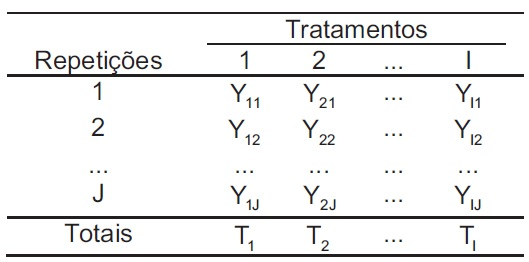
\includegraphics[scale=0.5]{Figuras/fig1}
    %\caption{}
    %\label{figRotulo}
  \end{figure}
\end{block}
\end{frame}

\begin{frame}{}
\frametitle{}
\begin{block}{}
\justifying
Deste quadro pode-se retirar algumas informações de interesse:
\begin{itemize}
\item Número de unidades experimentais: $N=I\times J$\pause
\item Total geral: $G={\displaystyle \sum_{i=1}^{I}\sum_{j=1}^{J}Y_{ij}=\sum_{i=1}^{I}T_{i}=Y_{\bullet \bullet}}$\pause
\item Total para o tratamento $i:\ T_{i}={\displaystyle \sum_{j=1}^{J}Y_{ij}=Y_{i\bullet}}$\pause
\item Média para o tratamento $i:\ \mu_{i}=\dfrac{T_{i}}{J}$\pause
\item Média geral do experimento: $\mu=\dfrac{G}{IJ}$
\end{itemize}
\end{block}
\end{frame}

\section{Modelo Estatístico}
\begin{frame}{Modelo Estatístico}
\frametitle{}
\begin{block}{}
\justifying
Existe um modelo estatístico específico para cada tipo de delineamento. O modelo
estatístico identifica quais são as fontes de variação dos valores de uma variável resposta em estudo. Para os dados oriundos de um experimento instalado segundo o DIC, o seguinte modelo estatístico deve ser utilizado nas análises estatísticas:
$$Y_{ij}=\mu+t_{i}+e_{ij}$$
em que, $Y_{ij}$ é o valor observado para a variável resposta obtido para o $i$-ésimo tratamento em sua $j$-ésima repetição; $\mu$ é a média de todos os valores possíveis da variável resposta; $t_{i}$ é o efeito do tratamento $i$ no valor observado $Y_{ij},$ ou seja, $t_{i}=\mu_{i}-\mu;$ Por fim, $e_{ij}$ é o erro experimental associado ao valor observado $Y_{ij},$ isto é, $e_{ij}=Y_{ij}-\mu_{i}.$
\end{block}
\end{frame}

\begin{frame}{}
\frametitle{}
\begin{block}{}
\justifying
O erro experimental ocorre em todos os experimentos, porque não é possível controlar o efeito de fontes de variações que ocorrem de forma aleatória e desconhecida. Este erro é o responsável pela variação observada entre as observações obtidas nas repetições para cada tratamento.
\end{block}
\end{frame}

\section{Análise de Variância}
\begin{frame}{Análise de Variância}
\frametitle{}
\begin{block}{}
\justifying
É uma técnica de análise estatística que permite decompor a variação total, ou
seja, a variação existente entre todas as observações, na variação devido à diferença
entre os efeitos dos tratamentos e na variação devido ao acaso, que também é
denominada de erro experimental ou resíduo.
\end{block}
\end{frame}

\begin{frame}{}
\frametitle{}
\begin{block}{}
\justifying
No entanto, para que esta técnica seja empregada é necessário que sejam
satisfeitas as seguintes pressuposições:
\begin{enumerate}
\item os efeitos do modelo estatístico devem ser aditivos;\pause
\item os erros experimentais devem ser normalmente distribuídos, independentes, com
média zero e com variância comum.
\end{enumerate}
Partindo do modelo estatístico, pode-se decompor a variação entre os valores
observados nas diferentes causas de variabilidade, como demonstrado a seguir.
\end{block}
\end{frame}

\begin{frame}{}
\frametitle{}
\begin{block}{}
\justifying
Considere o modelo estatístico para um experimento instalado segundo o DIC:
$$Y_{ij}=\mu+t_{i}+e_{ij}$$\pause
Fazendo $t_{i}=\mu_{i}-\mu$ e $e_{ij}=Y_{ij}-\mu_{i},$ tem-se:\pause
$$Y_{ij}-\mu=(\mu_{i}-\mu)+(Y_{ij}-\mu_{i}),$$\pause
Substituindo $\mu,\mu_{i}$ e $e_{ij}$ por seus estimadores tem-se:\pause
$$Y_{ij}-\hat{\mu}=(\hat{\mu}_{i}-\hat{\mu})+(Y_{ij}-\hat{\mu}_{i}),$$
\end{block}
\end{frame}

\begin{frame}{}
\frametitle{}
\begin{block}{}
\justifying
elevando ambos os membros ao quadrado e aplicando o somatório, temos:
$${\displaystyle \sum_{i=i,j=1}^{I,J}(Y_{ij}-\hat{\mu})^{2}=\sum_{i=i,j=1}^{I,J}\left[(\hat{\mu}_{i}-\hat{\mu})+(Y_{ij}-\hat{\mu}_{i})\right]^{2}}$$
$$\Rightarrow{\scriptsize{\displaystyle \sum_{i=i,j=1}^{I,J}(Y_{ij}-\hat{\mu})^{2}=\sum_{i=i,j=1}^{I,J}(\hat{\mu}_{i}-\hat{\mu})^{2}+\sum_{i=i,j=1}^{I,J}(Y_{ij}-\hat{\mu}_{i})^{2}+\sum_{i=i,j=1}^{I,J}\textrm{duplos produtos}}}$$
É fácil mostrar que ${\displaystyle \sum_{i=i,j=1}^{I,J}\textrm{duplos produtos}=0.}$ Logo, podemos escrever, simplificadamente:
$$SQTotal=SQTrat+SQRes$$
\end{block}
\end{frame}

\begin{frame}{}
\frametitle{}
\begin{block}{}
\justifying
Por meio destas fórmulas, pode-se obter os valores para as respectivas somas de quadrados. No entanto, essas fórmulas demandam muitos cálculos. Fórmulas de mais fácil aplicação podem ser obtidas, conforme é mostrado a seguir. Inicialmente trabalharemos com a fórmula da SQTotal. Tem-se:
$$SQTotal={\displaystyle \sum_{i=i,j=1}^{I,J}(Y_{ij}-\hat{\mu})^{2}}$$\pause
Desenvolvendo o quadrado perfeito,
$${\displaystyle \sum_{i=i,j=1}^{I,J}(Y_{ij}-\hat{\mu})^{2}=\sum_{i=i,j=1}^{I,J}(Y_{ij}^{2}-2\hat{\mu}Y_{ij}+\hat{\mu}^{2})}$$
\end{block}
\end{frame}

\begin{frame}{}
\frametitle{}
\begin{block}{}
\justifying
aplicando-se as propriedades de somatório, temos:
\begin{align}
{\displaystyle \sum_{i=i,j=1}^{I,J}(Y_{ij}-\hat{\mu})^{2}}&=
{\displaystyle \sum_{i=i,j=1}^{I,J}Y_{ij}^{2}-2\hat{\mu}\sum_{i=i,j=1}^{I,J}Y_{ij}+\sum_{i=i,j=1}^{I,J}\hat{\mu}^{2}}\\
&={\displaystyle \sum_{i=i,j=1}^{I,J}Y_{ij}^{2}-2\hat{\mu}\sum_{i=i,j=1}^{I,J}Y_{ij}+IJ\hat{\mu}^{2}}
\end{align}
\end{block}
\end{frame}

\begin{frame}{}
\frametitle{}
\begin{block}{}
\justifying
Sabemos que $\hat{\mu}=\dfrac{{\displaystyle \sum_{i=i,j=1}^{I,J}Y_{ij}}}{IJ},$ assim:
$$
{\displaystyle \sum_{i=i,j=1}^{I,J}(Y_{ij}-\hat{\mu})^{2}}=
{\displaystyle \sum_{i=i,j=1}^{I,J}Y_{ij}^{2}-2\left(\dfrac{{\displaystyle \sum_{i=i,j=1}^{I,J}Y_{ij}}}{IJ}\right)\sum_{i=i,j=1}^{I,J}Y_{ij}+IJ\left(\dfrac{{\displaystyle \sum_{i=i,j=1}^{I,J}Y_{ij}}}{IJ}\right)^{2}}
$$
\end{block}
\end{frame}

\begin{frame}{}
\frametitle{}
\begin{block}{}
\justifying
simplificando tem-se,
$$
{\displaystyle \sum_{i=i,j=1}^{I,J}(Y_{ij}-\hat{\mu})^{2}}=
{\displaystyle \sum_{i=i,j=1}^{I,J}Y_{ij}^{2}-2\dfrac{\left({\displaystyle \sum_{i=i,j=1}^{I,J}Y_{ij}}\right)^{2}}{IJ}+\dfrac{\left({\displaystyle \sum_{i=i,j=1}^{I,J}Y_{ij}}\right)^{2}}{IJ}}
$$
\end{block}
\end{frame}

\begin{frame}{}
\frametitle{}
\begin{block}{}
\justifying
Finalmente, temos:
$$
SQTotal={\displaystyle \sum_{i=i,j=1}^{I,J}(Y_{ij}-\hat{\mu})^{2}}=
{\displaystyle \sum_{i=i,j=1}^{I,J}Y_{ij}^{2}-\dfrac{\Biggl({\displaystyle \sum_{i=i,j=1}^{I,J}Y_{ij}}\Biggl)^{2}}{IJ}}
$$
que é a fórmula mais prática para se calcular a SQTotal.
\end{block}
\end{frame}

\begin{frame}{}
\frametitle{}
\begin{block}{}
\justifying
Para a SQTratamentos tem-se:
$$SQTrat={\displaystyle \sum_{i=1,j=1}^{I,J}(\hat{\mu}_{i}-\hat{\mu})^{2}}$$\pause
desenvolvendo o quadrado perfeito,
$${\displaystyle \sum_{i=1,j=1}^{I,J}(\hat{\mu}_{i}-\hat{\mu})^{2}}=
{\displaystyle \sum_{i=1,j=1}^{I,J}(\hat{\mu}_{i}^{2}-2\hat{\mu}\hat{\mu}_{i}+\hat{\mu}^{2})}$$
\end{block}
\end{frame}

\begin{frame}{}
\frametitle{}
\begin{block}{}
\justifying
aplicando-se as propriedades de somatório, temos:
\begin{align}
{\displaystyle \sum_{i=i,j=1}^{I,J}(\hat{\mu}_{i}-\hat{\mu})^{2}}&=
{\displaystyle \sum_{i=i,j=1}^{I,J}\hat{\mu}_{i}^{2}-2\hat{\mu}\sum_{i=i,j=1}^{I,J}\hat{\mu}_{i}+\sum_{i=i,j=1}^{I,J}\hat{\mu}^{2}}\\
&={\displaystyle J\sum_{i=i}^{I}\hat{\mu}_{i}^{2}-2\hat{\mu}J\sum_{i=i}^{I}\hat{\mu}_{i}+IJ\hat{\mu}^{2}}
\end{align}
\end{block}
\end{frame}

\begin{frame}{}
\frametitle{}
\begin{block}{}
\justifying
A média geral e a média para tratamentos podem ser escritas respectivamente como:
$$\hat{\mu}=\dfrac{{\displaystyle \sum_{i=i,j=1}^{I,J}Y_{ij}}}{IJ}\ \textrm{e}\ 
\hat{\mu}_{i}=\dfrac{T_{i}}{J}$$
Substituindo na expressão anterior, tem-se:
\begin{align*}
{\displaystyle \sum_{i=i,j=1}^{I,J}(\hat{\mu}_{i}-\hat{\mu})^{2}}&={\displaystyle J\sum_{i=i}^{I}\dfrac{T_{i}^{2}}{J^{2}}-2\left(\dfrac{{\displaystyle \sum_{i=i,j=1}^{I,J}Y_{ij}}}{IJ}\right)J\sum_{i=i}^{I}\dfrac{T_{i}}{J}+IJ\left(\dfrac{{\displaystyle \sum_{i=i,j=1}^{I,J}Y_{ij}}}{IJ}\right)^{2}}
\end{align*}
\end{block}
\end{frame}

\begin{frame}{}
\frametitle{}
\begin{block}{}
\justifying
Sabe-se que $T_{i}={\displaystyle \sum_{j=1}^{J}Y_{ij}},$ então:

\begin{center}
\scalebox{0.9}{%
$
{\displaystyle \sum_{i=i,j=1}^{I,J}(\hat{\mu}_{i}-\hat{\mu})^{2}}=
{\displaystyle J\sum_{i=i}^{I}\dfrac{T_{i}^{2}}{J^{2}}-2\left(\dfrac{{\displaystyle \sum_{i=i,j=1}^{I,J}Y_{ij}}}{IJ}\right)J\left(\dfrac{{\displaystyle\sum_{j=1}^{J}Y_{ij}}}{J}\right)+IJ\left(\dfrac{{\displaystyle \sum_{i=i,j=1}^{I,J}Y_{ij}}}{IJ}\right)^{2}}
$
}
\end{center}
\end{block}
\end{frame}

\begin{frame}{}
\frametitle{}
\begin{block}{}
\justifying
simplificando, tem-se:
\begin{center}
\scalebox{0.9}{%
$
{\displaystyle \sum_{i=i,j=1}^{I,J}(\hat{\mu}_{i}-\hat{\mu})^{2}}=
{\displaystyle \sum_{i=i}^{I}\dfrac{T_{i}^{2}}{J}-2\dfrac{\left({\displaystyle \sum_{i=i,j=1}^{I,J}Y_{ij}}\right)^{2}}{IJ}+\dfrac{{\displaystyle \left(\sum_{i=i,j=1}^{I,J}Y_{ij}\right)}^{2}}{IJ}}
$
}
\end{center}
finalmente tem-se:
$$
SQTrat={\displaystyle \sum_{i=i,j=1}^{I,J}(\hat{\mu}_{i}-\hat{\mu})^{2}}=
{\displaystyle \sum_{i=i}^{I}\dfrac{T_{i}^{2}}{J}-\dfrac{\left({\displaystyle \sum_{i=i,j=1}^{I,J}Y_{ij}}\right)^{2}}{IJ}}
$$
\end{block}
\end{frame}

\begin{frame}{}
\frametitle{}
\begin{block}{}
\justifying
A fórmula anterior é utilizada quando o número de repetições é igual para todos os
tratamentos. No caso em que o número de repetições varia de acordo com o tratamento a
fórmula apropriada é:
$$
SQTrat=
{\displaystyle \sum_{i=i}^{I}\dfrac{T_{i}^{2}}{r_{i}}-\dfrac{\left({\displaystyle \sum_{i=i,j=1}^{I,r_{i}}Y_{ij}}\right)^{2}}{N}}
$$
em que, $N$ é o número de unidades experimentais $={\displaystyle \sum_{i=1}^{I}r_{i}},$ e $r_{i}$ é número de unidades experimentais do tratamento $i.$
\end{block}
\end{frame}

\begin{frame}{}
\frametitle{}
\begin{block}{}
\justifying
Por fim, A Soma de Quadrados do Resíduo $(SQRes)$ é obtida por diferença,
$$SQRes=SQTotal-SQTrat$$
\end{block}
\end{frame}

\begin{frame}{}
\frametitle{}
\begin{block}{}
\justifying
O quadro da análise de variância, geralmente denotada por ANOVA (ANalysis Of
VAriance) para a análise de um experimento instalado segundo o DIC, com igual número
de repetições para todos os tratamentos é do seguinte tipo:
\begin{table}[!h]
\scalebox{0.9}{%
\setlength{\arrayrulewidth}{2pt}
\begin{tabular}{cccccc}
\hline
FV&GL&SQ&QM&F&$F_{tab;\alpha}$\\
\hline
&&&&&\\
Tratamentos&$(I-1)$&SQTrat&$\dfrac{SQTrat}{I-1}$&$\dfrac{QMTrat}{QMRes}$&$[(I-1);I(J-1)]$\\
&&&&&\\
Resíduo&$I(J-1)$&SQRes&$\dfrac{SQRes}{I(J-1)}$&&\\
\hline
Total&IJ-1&SQTotal&&&\\
\hline
\end{tabular}
}
\end{table}
\end{block}
\end{frame}

\begin{frame}{}
\frametitle{}
\begin{block}{}
\justifying
A partir das $SQTrat$ e $SQRes,$ obtém-se os respectivos quadrados médios, por
meio do quociente entre a soma de quadrados com o respectivo número de graus de
liberdade.
\end{block}
\pause
\begin{block}{}
\justifying
Para se concluir se existe diferença entre tratamentos, calcula-se o valor de F, que
é obtido pelo quociente do $QMTrat$ com o $QMRes.$ Este valor de F calculado deve ser
comparado com o valor de F tabelado, o qual é obtido na tabela de distribuição da
variável aleatória F, de acordo com o nível de significância do teste, graus de liberdade para tratamentos e graus de liberdade para resíduo.
\end{block}
\end{frame}

\begin{frame}{}
\frametitle{}
\begin{block}{}
\justifying
As hipóteses para o teste F da análise de variância para tratamentos são as
seguintes:
$H_{0}:\mu_{1}=\cdots=\mu_{I}=\mu$, o que equivale a dizer que todos os possíveis contrastes entre as médias dos tratamentos, são estatisticamente nulos, ao nível de
probabilidade que foi executado o teste.\pause
$H_{a}:\textrm{não}\ H_{0},$ o que equivale a dizer que existe pelo menos um contraste entre as médias dos tratamentos, estatisticamente diferentes de zero, ao nível de probabilidade que foi realizado o teste.
\end{block}
\end{frame}

\begin{frame}{}
\frametitle{}
\begin{block}{}
\justifying
A regra decisória para o teste F é a seguinte:
\begin{itemize}
\item Se o valor do F calculado for maior ou igual ao valor do F tabelado, então rejeita-se $H_{0}$ e conclui-se que os tratamentos tem efeito diferenciado ao nível de significância em que foi realizado o teste;\pause
\item Se o valor de F calculado for menor que o valor do F tabelado, então não rejeita-se $H_{0}$ e conclui-se que os tratamentos têm efeitos iguais ao nível de significância em que foi realizado o teste.
\end{itemize}
\end{block}
\end{frame}

\section{Coeficiente de Variação}
\begin{frame}{Coeficiente de Variação}
\frametitle{}
\begin{block}{}
\justifying
O coeficiente de variação é calculado da seguinte maneira:
$$CV=\dfrac{\sqrt{QMRes}}{\hat{\mu}}.100$$
O CV é utilizado para avaliação da precisão de experimentos. Quanto menor o CV
mais preciso tende a ser o experimento.
\end{block}
\end{frame}

\begin{frame}{}
\frametitle{Vantagens e Desvantagens do delineamento inteiramente casualizado}
\begin{block}{Vantagens:}
\begin{itemize}
\item Não existem exigências quanto ao número de tratamentos e repetições;\pause
\item É o delineamento com maior valor para os graus de liberdade do resíduo.
\end{itemize}
\end{block}
\pause
\begin{block}{Desvantagens:}
\begin{itemize}
\item Não é fácil conseguir e manter total homogeneidade das condições;\pause
\item todas as variações exceto a devida a tratamentos, são consideradas aleatórias. Isto pode acarretar uma estimativa muito alta para o erro experimental.
\end{itemize}
\end{block}
\end{frame}

\section{Exemplos}
\begin{frame}{}
\frametitle{}
\begin{block}{}
\justifying
Para comparar a produtividade de quatro variedades de milho, um agrônomo tomou
vinte parcelas similares e distribuiu, inteiramente ao acaso, cada uma das 4 variedades
em 5 parcelas experimentais. A partir dos dados experimentais fornecidos, é possível concluir que existe diferença significativa entre as variedades com relação a 
produtividade, utilizando o nível de significância de $5\%?$
\begin{table}[!h]
\scalebox{0.8}{%
\setlength{\arrayrulewidth}{2pt}
\begin{tabular}{ccccc}
\hline
\multicolumn{5}{c}{{\bf Variedades}}\\
\hline
&A&B&C&D\\
\hline
&25&31&22&33\\
&26&25&26&29\\
&20&28&28&31\\
&23&27&25&34\\
&21&24&29&28\\
\hline
Totais&115&135&130&155\\
\hline
Médias&23&27&26&31\\
\hline
\end{tabular}
}
\end{table}
\nocite{calegare}
\nocite{ivo}
\end{block}
\end{frame}

\begin{frame}[allowframebreaks]
\frametitle{Referências Bibliográficas}
\bibliography{bibliografia}
\end{frame}

\end{document}
